\chapter{A new mouse model of FUS-mediated ALS}
\label{chapter:fus_mouse}

Work presented in this chapter has been published as part of \citep{Devoy2017}. See appendices for full reproduction of the published manuscript.


\section{Overview}
This chapter describes work carried out in collaboration with Dr Anny Devoy of the UCL Institute of Neurology. Dr Devoy has created a "humanised" mouse model of ALS resulting from a mutation in the FUS RNA-binding protein. 

\section{Background}
% REWRITE
All previous studies alter FUS expression to levels that wildly differ to the normal biological situation. Overexpression or knockout are clearly toxic but these do not help to differentiate the effects of the mutations of normal FUS function. Until now there have been no studies where the effects of a human FUS mutation are seen on the mouse at a physiological level of expression. 
The FUS $\Delta$14 mutation was found in an early onset ALS patient who died at the age of 22 following a very rapid disease course \citep{DeJesus-Hernandez2010}. The mutation alters the 3' splice site of exon 14 of FUS, causing it to be skipped.  Comparison of the $\Delta$14 mutation with other, late-onset ALS causing mutations have shown an increased propensity by FUS $\Delta$14 to accumulate in the cytoplasm \citep{Verbeeck2012}. Analysis of mice carrying a single copy of the FUS $\Delta$14 mutation enables a reconstruction of progressive neurodegenerative disease. By analysing RNA-seq data collected across the lifespan of the mice, I can observe specific RNA dysregulation due to the mutant protein.


\subsection{Aims of the project}
My role within the project was to analyse RNA sequencing data comparing the FUS $\Delta$14 mice with their wildtype littermates across two tissues and timepoints. The project so far has only looked at gene expression but the eventual aim is to carefully look at splicing changes.


\section{Contributions}
\begin{itemize}
	% Check with Pietro
	\item Transgenic mice were created by Dr Anny Devoy
	\item RNA sequencing libraries were prepared by Dr Anny Devoy
	\item RT-PCR validation was performed by Dr Anny Devoy
	\item Figure \ref{fig:delta14_structure} was created by Dr Anny Devoy
\end{itemize}
All bioinformatic analysis and interpretation was designed and performed by myself in consultation with Dr Anny Devoy and my supervisors. 




%%FUS overexpression causes neurodegeneration and FUS-positive inclusions, cytoplasmic FUS expression in mice \citep{Mitchell2013} although only in homozygous state (dose sensitive) hemizygous FUS overexpression shows no evidence of motor phenotype

%
%\citep{Verbeeck2012} wildtype or mutant human FUS expressed in mouse brain (one mutant is delta14). Both mutants accumulate in cytoplasm with delta14 showing strongest changes with insoluble FUS cytoplasmic inclusions, although no neurodegeneration was observed within the 3 month time frame 

%\citep{Scekic-zahirovic2016} created mice with knockin mutant FUS and knockout FUS. Both show perinatal lethality and splicing changes - mislocalisation results in loss of normal function. BUT only the mutant knockin mice show reduced motor neurons at birth, which can be rescued by cell specific WT FUS expression. Toxic gain of function?
%dupuis paper - compared reversible truncation with FUS knockout in homozygous state - both show perinatal lethality but only FUS knockin demonstrated reduced motor neuron number
%
%\citep{Sharma2016} Single copy of WT or ALS mutant FUS is expressed from MApT locus conditionally in mice, had an adult onset and a juvenile onset mutation. Conditional FUS knockout post-natal does not affect long term survival of motor neurons - toxic gain of function. Combining both demonstrated that mutant FUS does not depend on WT FUS to induce toxic aggregates. Mutant FUS was more highly expressed than wildtype - more stable.
%
%Issues - expression levels are not physiological - overexpression of FUS can cause degeneration but not realistic in disease.
%
%%Human FUS in overexpressed in adult rats, progressive motor impairment and respiratory dysfunction \citep{Jackson2016}

\subsection{The FUS $\Delta$14 mouse is a humanised model of ALS}
The FUS $\Delta$14 mouse was created by directed mutagenesis of the mouse Fus exon 14 splice site as well as humanisation of exon 15 with 4 separate mutations.The result of splicing exons 13 and 15 together is a frameshift which at the protein level removes the C-terminal nuclear localisation signal (Figure 4.1A) but leaves a novel peptide sequence which can used to create specific antibodies. Reverse-transcription PCR to detect FUS mRNA showed the $\Delta$14 FUS mRNA to be expressed at a similar level to wildtype FUS (Fig. \ref{fig:delta14_structure}B). 


\begin{table}[h!]
	\caption{All RNA-sequencing data used in this study}
	Library info describes the type of library prepared, the length of each read and whether the sequencing was single or paired end. PE: paired end sequencing. Depth is defined the number of uniquely mapped read pairs, in millions.
	\begin{center}
		\begin{small}
			\begin{tabular}{llllp{1.5cm}llll}
				Species & Cell type & Time point & Library info & Depth & Number\\
				\hline
				Mouse & Spinal Cord & 3 months & stranded mRNA 75bp PE & 33-43M & 4 vs 4\\
				Mouse & Spinal Cord & 12 months & stranded mRNA 75bp PE & 35-46M & 4 vs 4\\ 
				Mouse & Motor/Frontal Cortex & 3 months & stranded mRNA 75bp PE & 35-52M & 4 vs 4\\
				Mouse & Motor/Frontal Cortex & 12 months & stranded mRNA 75bp PE & 35-48M & 4 vs 4\\ 
			\end{tabular}
		\end{small}
	\end{center}
\end{table}

\begin{figure}[h!]
	\begin{center}
		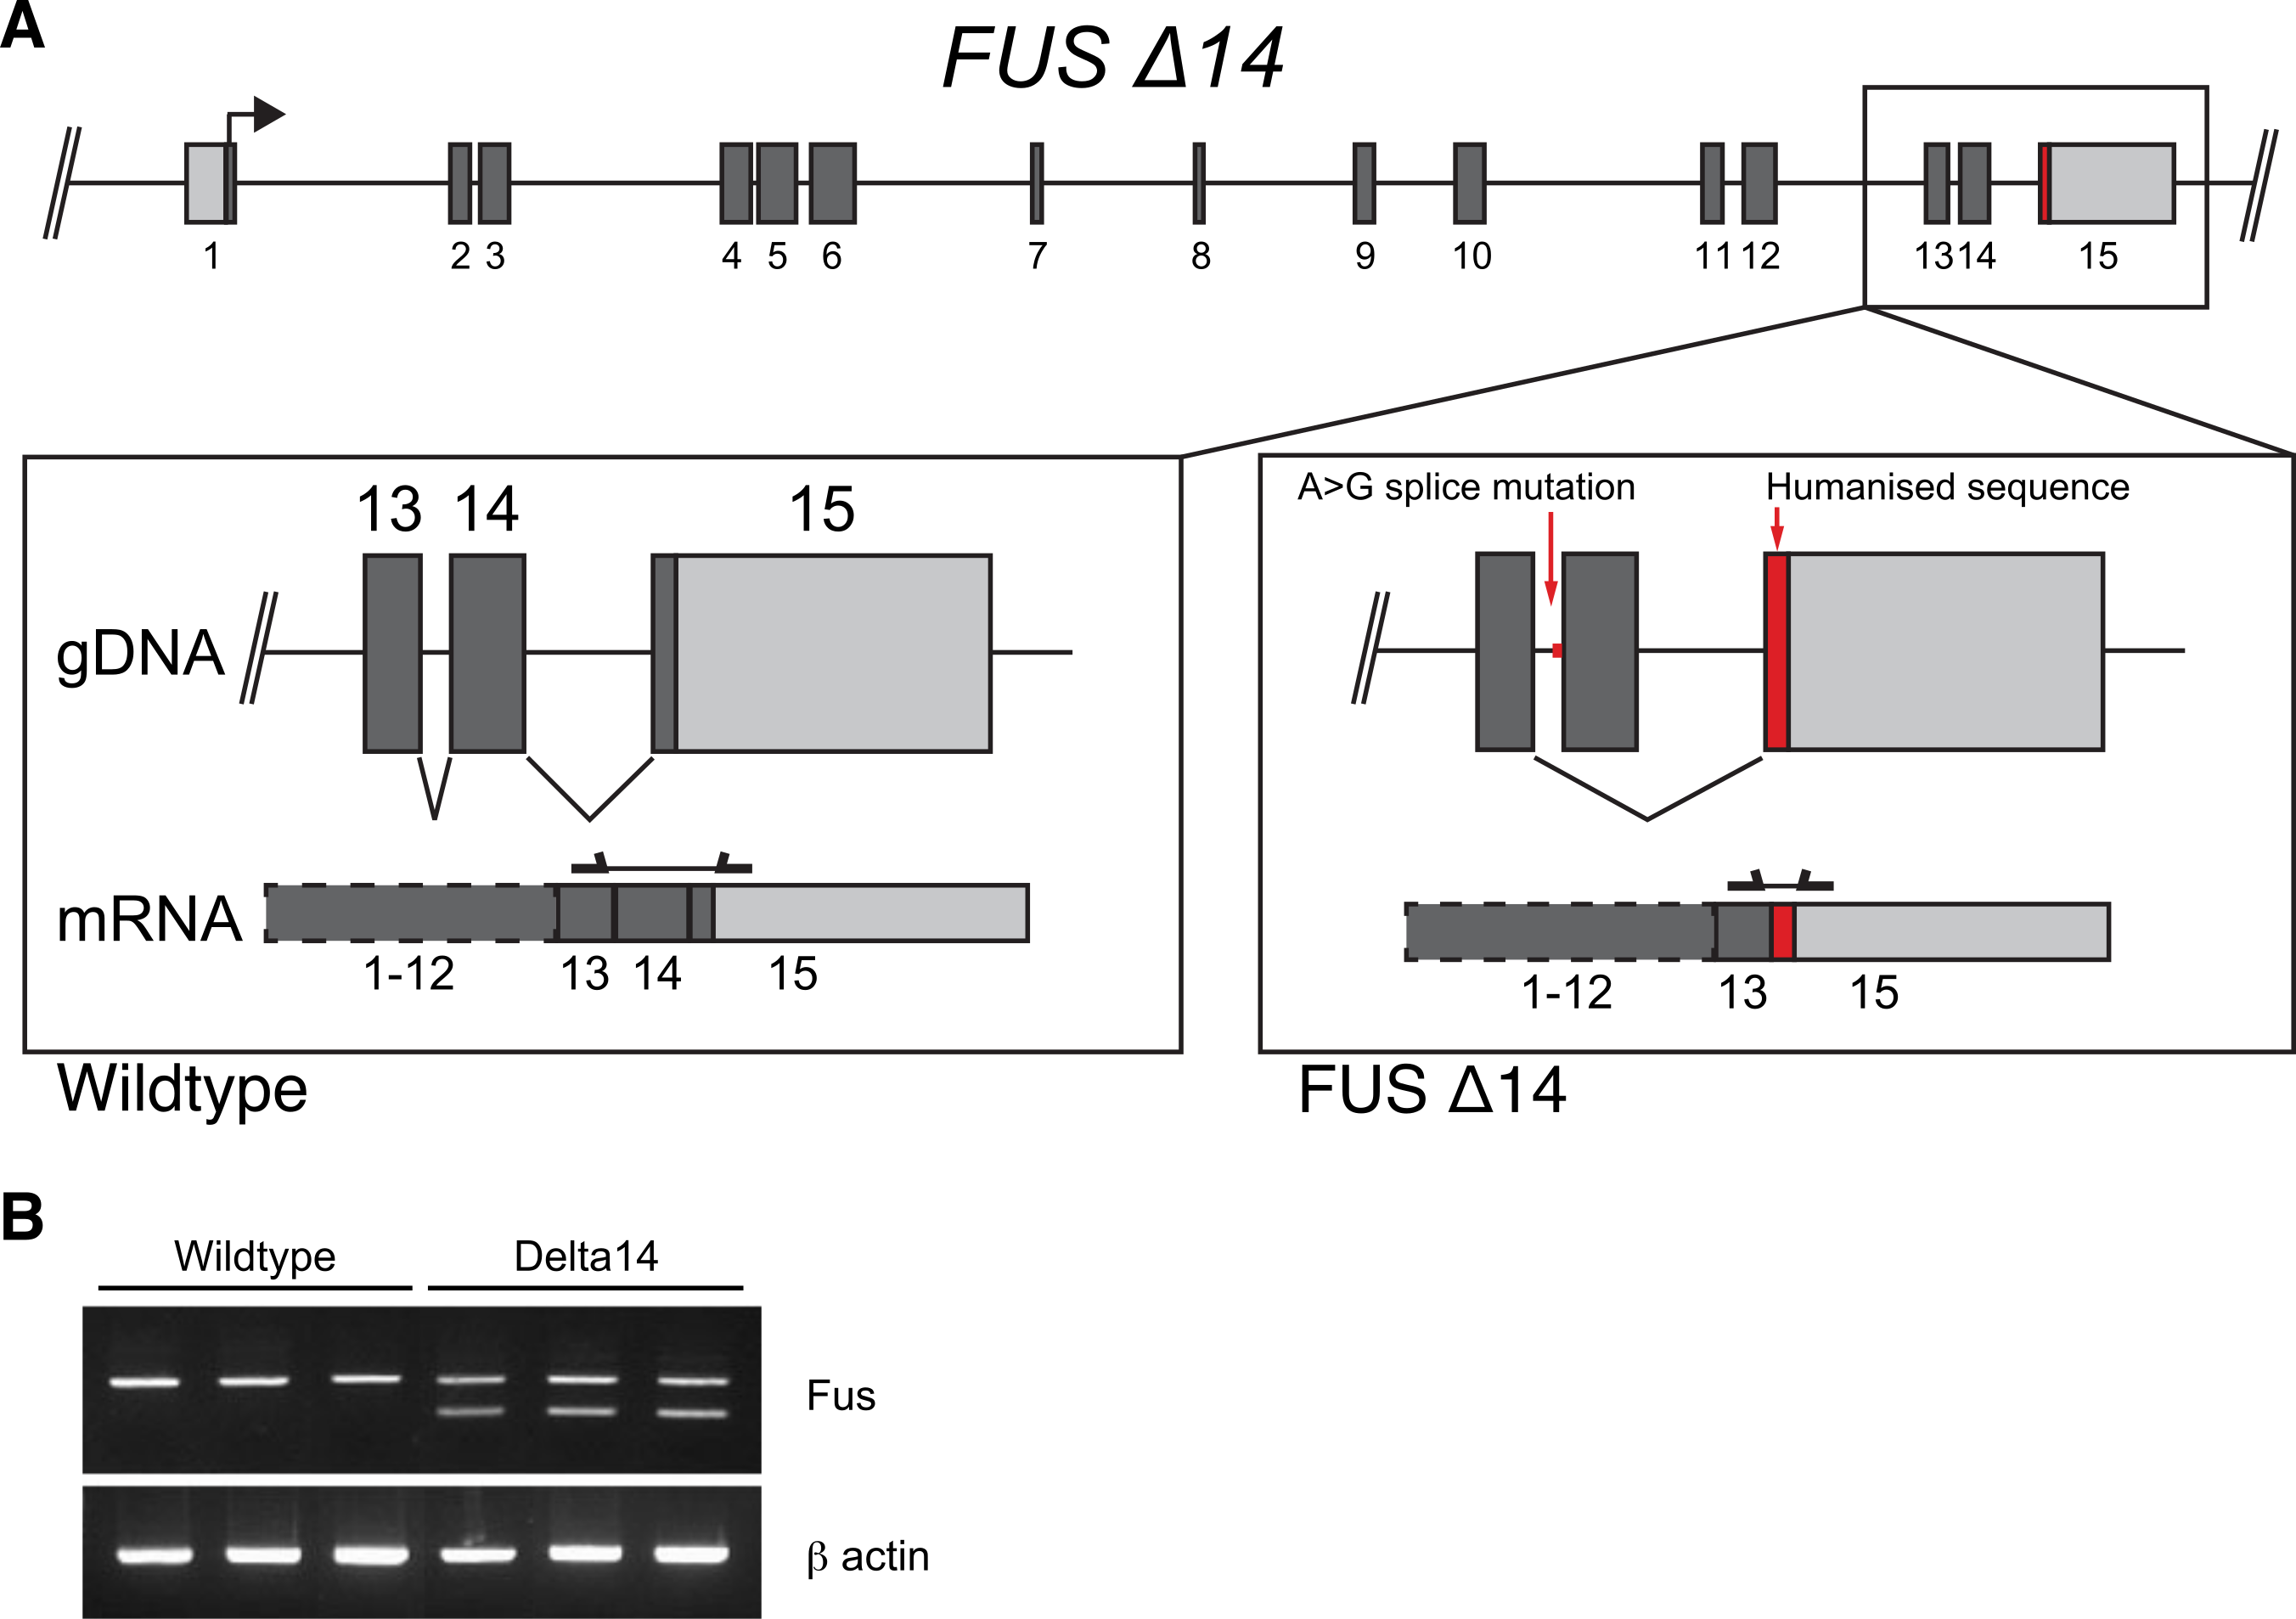
\includegraphics[width=\textwidth]{Figures/04_fus_mice/anny_FUS_schematic.png}
	\end{center}
	\caption{\textbf{The FUS $\Delta$14 model} }
		A) The FUS locus with a closeup of the terminal three exons in the wildtype mouse (left) and the FUS $\Delta$14 mouse (right) B) RT-PCR of FUS mRNA from spinal cord of wildtype and mutant mice. \textit{Figure created by Anny Devoy}
			\label{fig:delta14_structure}
\end{figure}


\section{Methods}

\subsection{Data preparation}
All RNA-seq data used is listed in table 4.1. All samples were aligned to the mm10 mouse reference genome using the previously discussed analysis pipeline.

\subsection{Differential gene expression}
Differential expression was carried out with \textit{DESeq2} \citep{Love2014} comparing wildtype with mutant mice. All P-values were adjusted at a false discovery rate of 10\%. To assess the variance between each sample the raw counts for each gene were normalised to account for library size and then normalised again by the regularized log normalisation method \citep{Love2014}. The counts were further transformed into Z-scores, which express the number of standard deviations from the mean of all counts for that gene. Heatmaps were created for all significantly differentially expressed genes using the \textit{pheatmap} R package \citep{Kolde2012}.  

\subsection{Gene Ontology analysis}
Gene ontology (GO) analysis is a method to extract inference from gene expression experiments by annotating each gene and protein within a unified vocabulary of molecular and cellular function. This can be used to identify dyregulated pathways or broader trends \citep{Ashburner2000}. For each differential expression results set the multiple correction threshold was dropped to P < 0.005 for each gene to increase the number of input genes. The resulting list of hits was then annotated for GO terms and a hypergeometric test was applied to test the enrichment of particular categories against a background set of genes. It is important to account for selection bias for long genes in RNA-seq data as longer genes have more power to be differentially expressed than shorter genes \citep{Young2010}. The R package \textit{GOseq} implements a GO term annotation and enrichment test which takes account of this length bias \citep{Young2010}. The resulting P-values were then Bonferroni corrected for multiple testing. In each category the number of genes that were up- or downregulated in the $\Delta$14 mice relative to wildtype littermates were expressed as a percentage. 

\section{Results}

\subsection{Gene expression changes are tissue- and time point-specific}

To examine progressive changes in RNA regulation, total RNA was extracted from both spinal cord and forebrain from mice across two time-points: 3 months and 12 months. Four male mice of each genotype ($\Delta$14 and wildtype littermate) were used at each timepoint. At 3 months of age, the forebrain and spinal cord samples had 1 and 3 genes differentially expressed respectively. At 12 months of age there were no differentially expressed genes found in the forebrain but 1,289 found in the spinal cord, with genes predominantly decreased in expression (Figure 4.2). To examine the variance between each sample in the 12 month spinal cord dataset, the read counts for each gene were normalised and converted to Z-score values. Plotted as a heatmap it is clear that the 4 samples of each category are highly variable (Figure 4.3).

\begin{figure}[h!]
	\begin{center}
		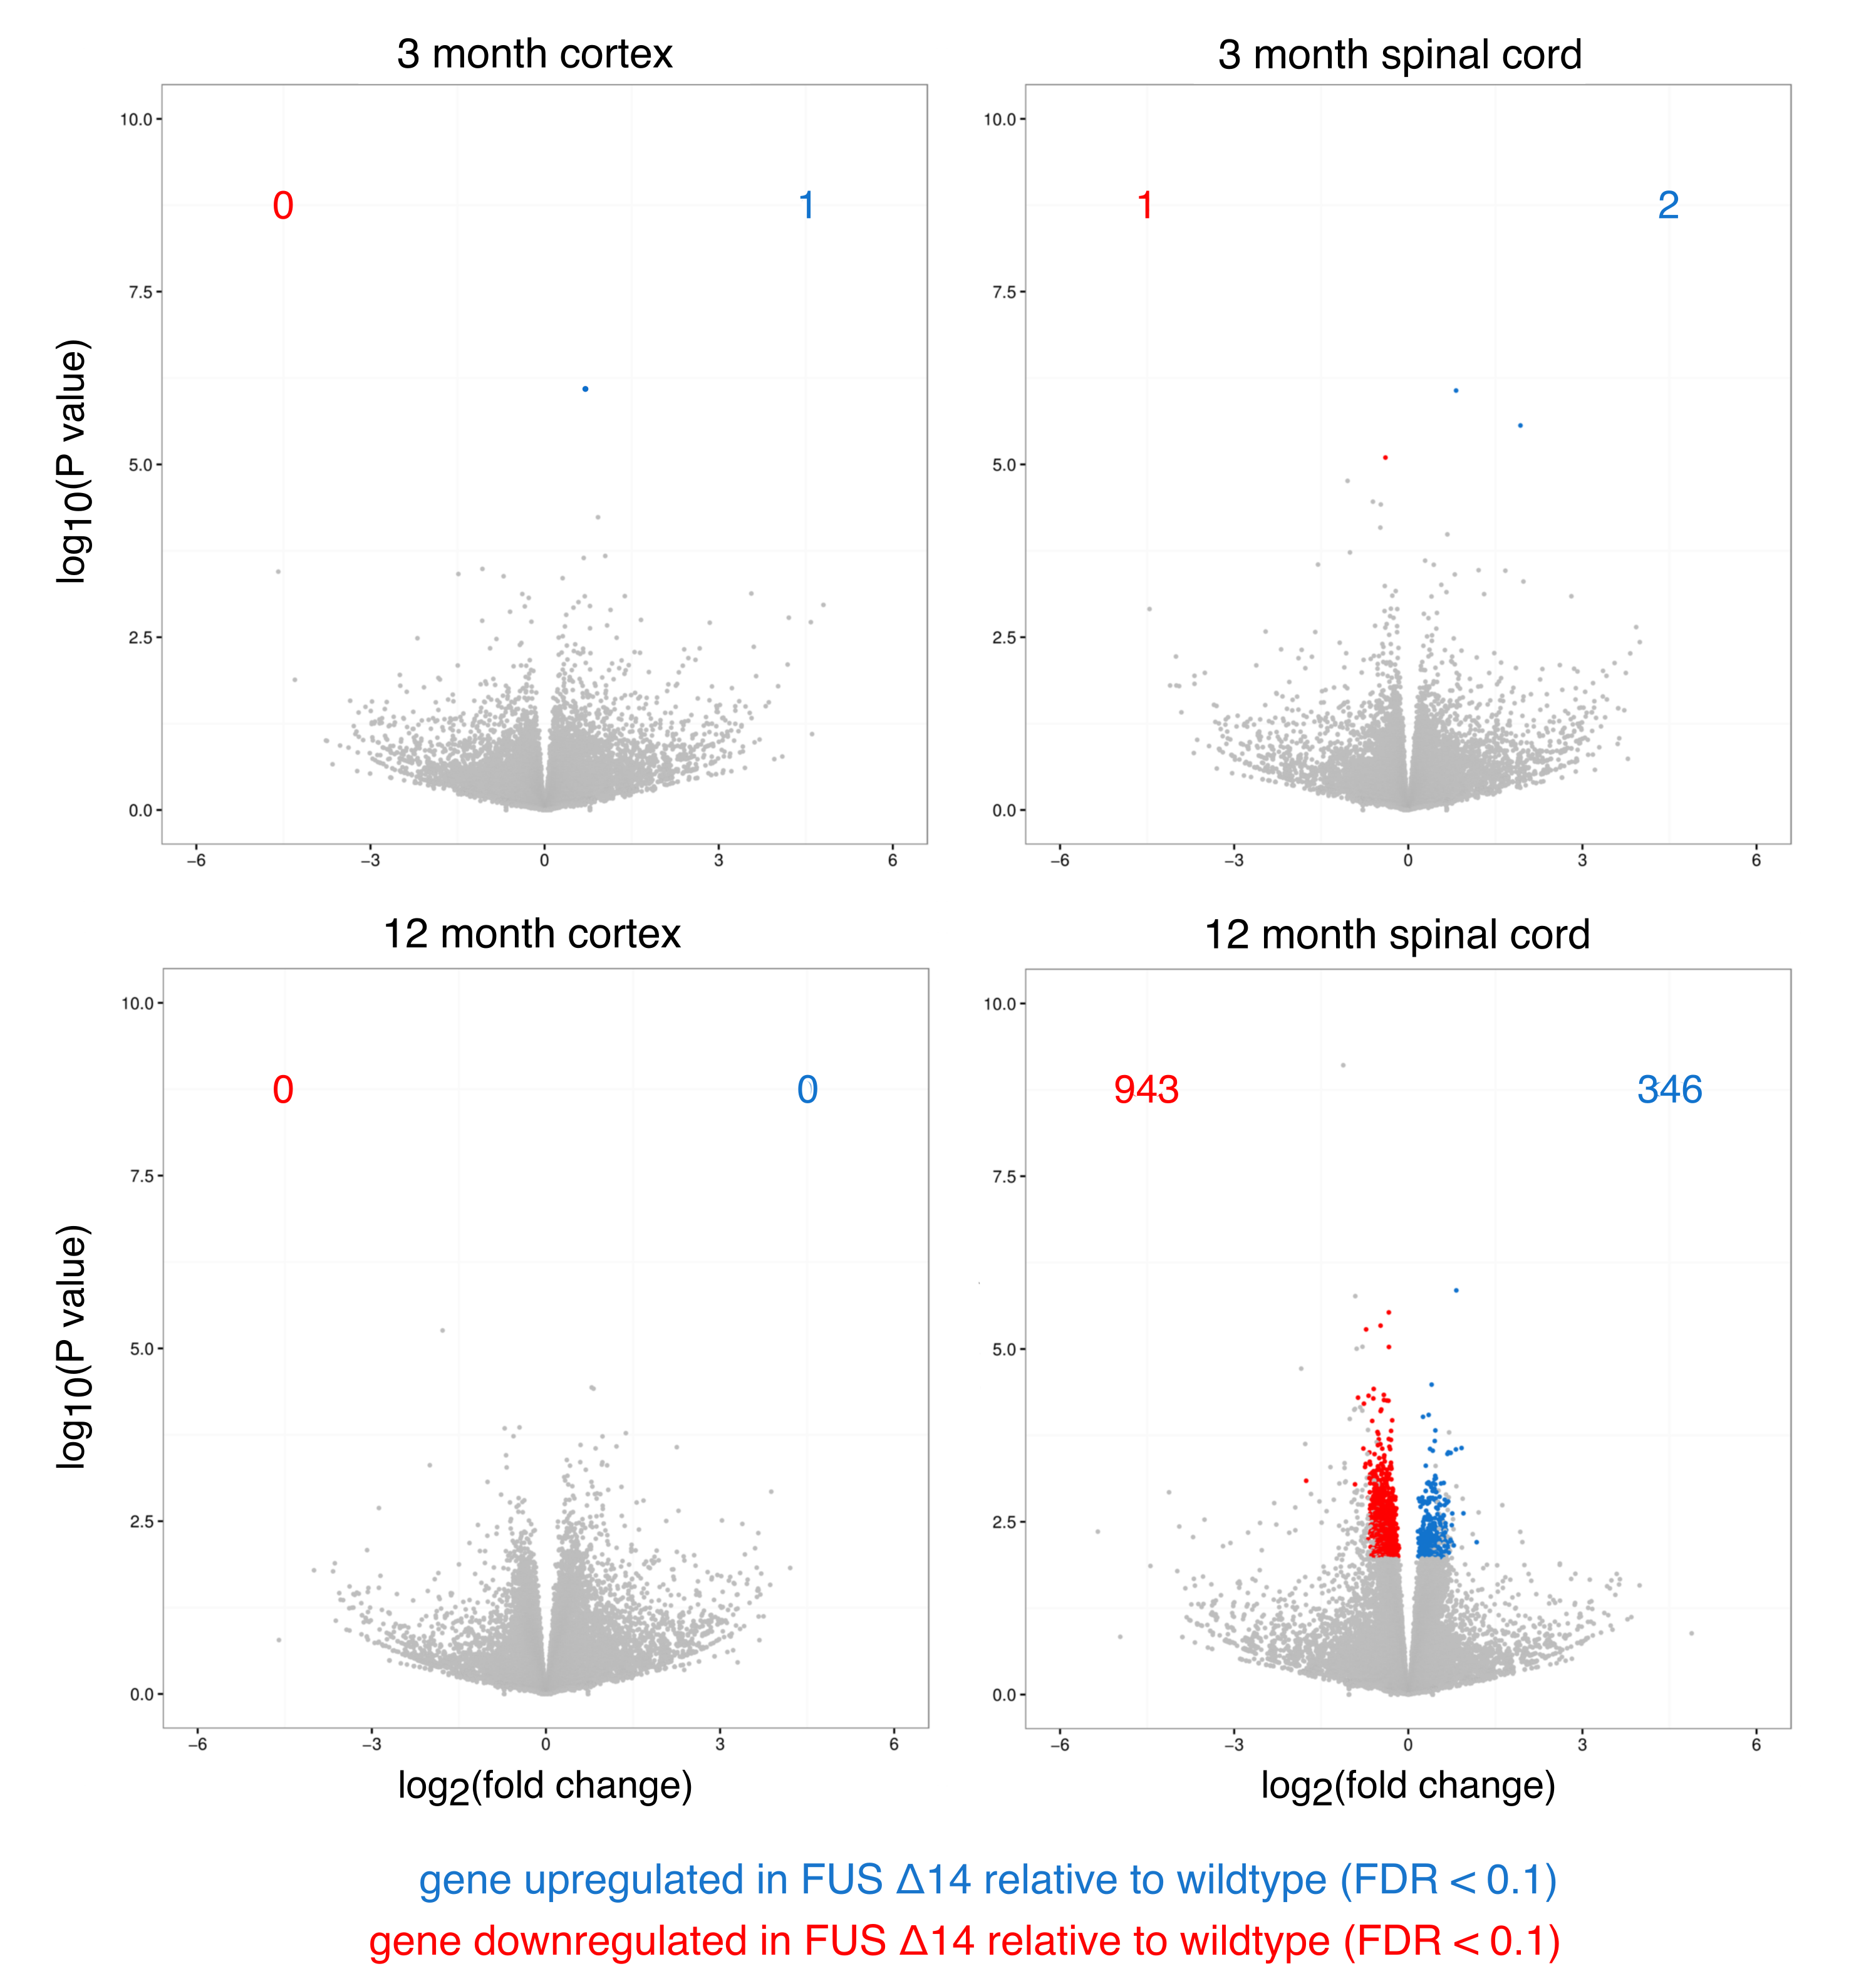
\includegraphics[width=\textwidth]{Figures/04_fus_mice/anny_volcanos.png}
	\end{center}
	\caption{Differential gene expression analysis on the $\Delta$14 mouse across two tissues and time points}
	Each gene is represented as a point. The x axis is the log2 of the ratio between the average expression in the $\Delta$14 mice against that of the wildtype mice. The y axis is the $log_10$ of the unadjusted P-value for the differential expression test. The numbers of upregulated genes (adjusted \textit{P} < 0.1 with a $log_2$(fold change) > 0) are in blue and the the downregulated ( adjusted \textit{P} < 0.1 with $log_2$(fold change) < 0) are in red.
	\label{fig:delta14_volcanos}
\end{figure}

\begin{figure}[h!]
	\begin{center}
		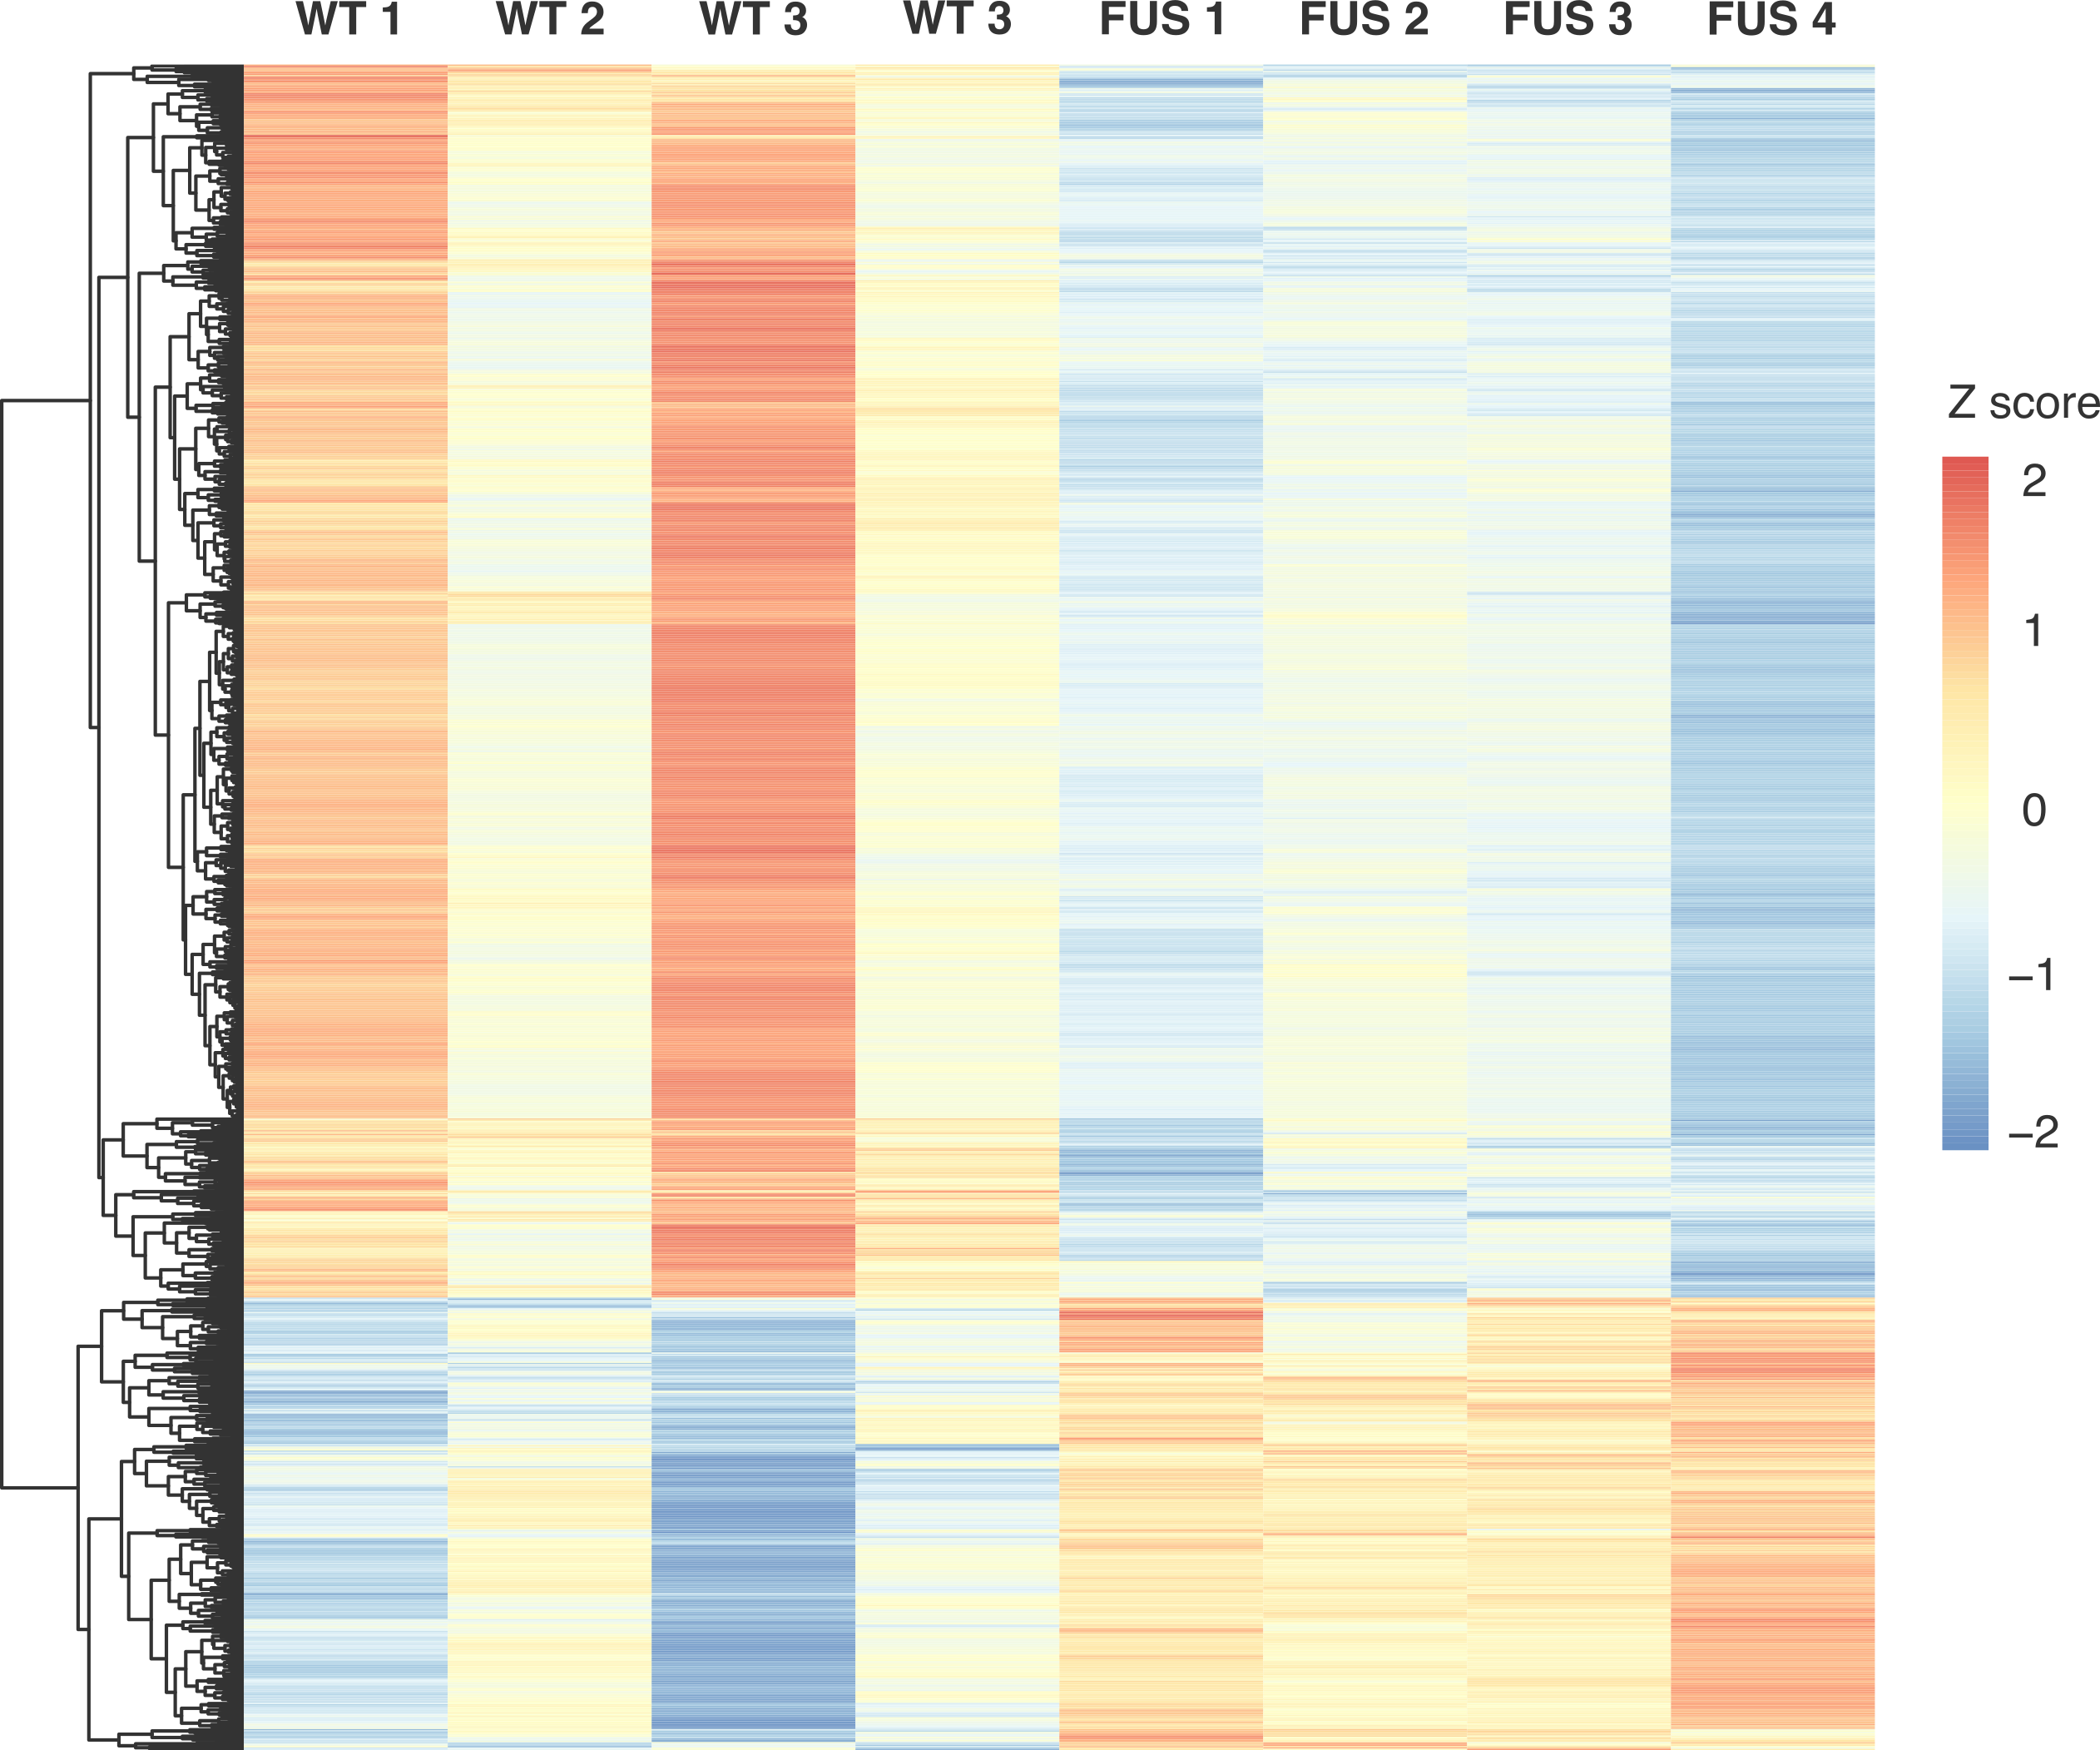
\includegraphics[width=\textwidth]{Figures/04_fus_mice/anny_normalised_heatmap.png}
	\end{center}
	\caption{\textbf{Z-score heatmap of the 1289 differentially expressed genes in 12 month spinal cord dataset}}
	WT: wildtype littermate; FUS: FUS $\Delta$14 heterozygote. 
\end{figure}


\subsection{Gene ontology analysis indicates changes in mitochondrial and ribosomal pathways}
Genes from the 12 month spinal cord dataset differentially expressed at a relaxed threshold of \textit{P} < 0.005 were sent for gene ontology enrichment analysis. This compares the number of genes that are members of a particular ontology category with the expected distribution. This analysis identified a strong enrichment in genes belonging to mitochondria, ribosome and proteasome cateogories. Strikingly, almost all the genes in these categories were downregulated (Figure 4.4).
\begin{figure}[h!]
	\begin{center}
		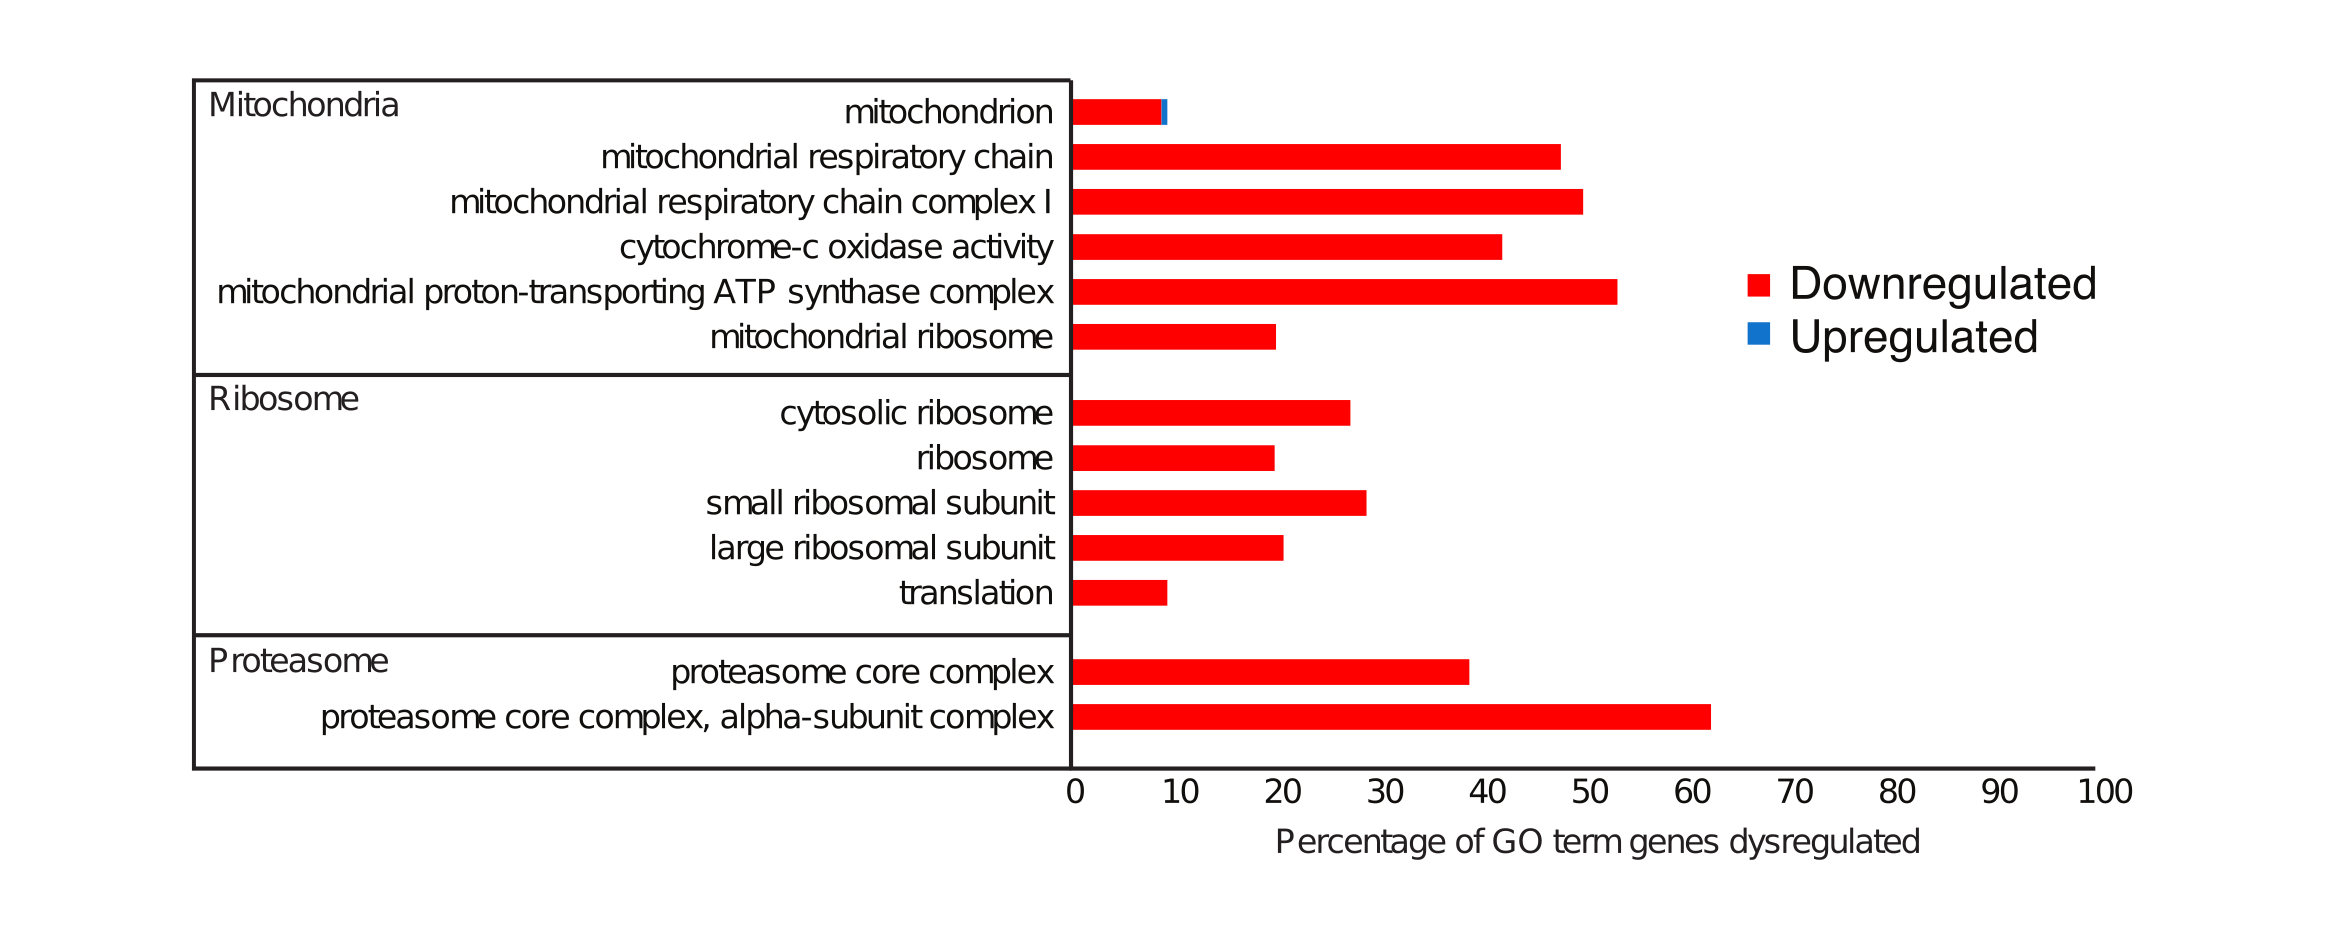
\includegraphics[width=12cm]{Figures/04_fus_mice/anny_GO_terms.png}
	\end{center}
	\caption{\textbf{Gene ontology categories significantly enriched in the 12 month FUS $\Delta$14 spinal cord samples}}
		Each significant gene ontology category ( adjusted P < 0.05) is expressed as a proportion of upregulated (red) or downregulated (blue) genes.
		\label{fig:delta14_go}
\end{figure}


\subsection{No splicing changes observed at 12 months beyond Fus itself}
I ran DEXSeq and SGSeq on the 12 month spinal cord samples. No convincing splicing changes were observed except for a cluster of splicing events in the FUS gene which are presumably a result of the mutation.


\section{Discussion}
My gene expression analysis demonstrates a progressive and tissue-specific change in RNA regulation, with 1,289 genes differentially expressed in the spinal cord of 12 month mutant mice. This finding is complemented by other contributions to the project. Behavioural experiments have shown the $\Delta$14 mice to have a progressive loss of motor function that is observable from 12 months of age. In addition, a reduction in number of motor neurons in the lumbar spinal cord has been observed from 12 months onwards, accompanied by an increase in cytoplasmic mislocalisation specifically of the mutant FUS.
The broad downregulation of mitochondrial, ribosomal and proteasomal genes specifically in the spinal cord of late-stage mice is an interesting finding that deserves further investigation. An enrichment of mitochondrial GO categories was previously seen in a FUS knockdown experiment conducted in human embryonic kidney cells  \citep{Schwartz2012}, suggesting that mitochondrial changes may be due to a loss of normal FUS function. A recent paper has identified mitochondrial defects in the brains of FTD-FUS patients and has shown FUS translocating to mitochondria \citep{Deng2015}, giving FUS an important role that may be perturbed by the $\Delta$14 mutation.
